%% if some package prevents compilation, remove it

\documentclass[a4paper, 11pt]{article}
\usepackage{fullpage}
\usepackage{titling}
\usepackage{graphicx}
\usepackage{xcolor}
\usepackage{amsmath}
\usepackage{amssymb}
\usepackage{amsthm}
\usepackage{hyperref}
\usepackage{IEEEtrantools} 
\usepackage{bbm}
\usepackage{lineno}
\usepackage{multirow}
\usepackage{longtable}
\usepackage{makecell}
\usepackage{lipsum}
\usepackage{etoolbox} %% <- for \pretocmd and \apptocmd
\usepackage{algorithm}
\usepackage[noend]{algpseudocode}
\usepackage{subfigure}

\setlength{\droptitle}{-6em}   % This is your set screw, for shifting up the title
\renewcommand{\baselinestretch}{1.1}
\setlength{\parskip}{0.5em}

\author{Aniket Sharma
  \\ December 17, 2023}
\date{}
\title{Statistical Query Learning \vspace{-0.5cm}}

\makeatletter %% <- make @ usable in macro names
\newcommand*\linenomathpatch{\@ifstar{\linenomathpatch@AMS}{\linenomathpatch@}}
\newcommand*\linenomathpatch@[1]{
  \expandafter\pretocmd\csname #1\endcsname {\linenomathWithnumbers}{}{}
  \expandafter\pretocmd\csname #1*\endcsname{\linenomathWithnumbers}{}{}
  \expandafter\apptocmd\csname end#1\endcsname {\endlinenomath}{}{}
  \expandafter\apptocmd\csname end#1*\endcsname{\endlinenomath}{}{}
}
\newcommand*\linenomathpatch@AMS[1]{
  \expandafter\pretocmd\csname #1\endcsname {\linenomathWithnumbersAMS}{}{}
  \expandafter\pretocmd\csname #1*\endcsname{\linenomathWithnumbersAMS}{}{}
  \expandafter\apptocmd\csname end#1\endcsname {\endlinenomath}{}{}
  \expandafter\apptocmd\csname end#1*\endcsname{\endlinenomath}{}{}
}
\let\linenomathWithnumbersAMS\linenomathWithnumbers
\patchcmd\linenomathWithnumbersAMS{\advance\postdisplaypenalty\linenopenalty}{}{}{}
\makeatother %% revert @
\linenomathpatch{IEEEeqnarray}
\linenomathpatch{equation}
\linenomathpatch*{gather}
\linenomathpatch*{multline}
\linenomathpatch*{align}
\linenomathpatch*{alignat}
\linenomathpatch*{flalign}

\usepackage{natbib}

\newtheorem{definition}{Definition}
\newtheorem{theorem}{Theorem}
\newtheorem{lemma}{Lemma}
\newtheorem{corollary}{Corollary}
\newtheorem{proposition}{Proposition}

\newcommand{\Prob}[1]{\mathbb{P}( #1 )}
\newcommand{\cA}{\mathcal{A}}
\newcommand{\E}{\mathbb E}
\newcommand{\EE}[1]{\E[#1]}
\newcommand{\cX}{\mathcal{X}}
\newcommand{\cY}{\mathcal{Y}}
\newcommand{\cZ}{\mathcal{Z}}
\newcommand{\cD}{\mathcal{D}}
\newcommand{\R}{\mathbb{R}}

\begin{document}
\maketitle
\vspace{-2cm}
\linenumbers

\section{Introduction}
Statistical Query (SQ) learning is a learning framework introduced by \cite{kearns_efficient_1998} for designing machine learning algorithms tolerant to white label noise (\cite{angluin_learning_1988}). It is originated from and is a restriction of the Probably Approximately Correct (PAC) learning model (\cite{valiant_theory_1984}) as it restricts the learning algorithm to use statistical properties of the data instead of a set of data samples.

The importance of SQ learning framework lies in its usefulness in defining robust and noise-tolerant learning algorithms. Virtually all noise-tolerant learning algorithms based on PAC model were either obtained from a SQ algorithm or any be captured by the SQ model with the noise rate approaching the information-theoretic barrier of 1/2 (\cite{kearns_efficient_1998}, \cite{feldman_statistical_2008}). SQ learning is also useful in a variety of modern applications like optimization (\cite{feldman_statistical_2017}), evolvability (\cite{feldman_evolvability_2008}), differential privacy (\cite{dwork_calibrating_2006}) and adaptive data analysis (\cite{dwork_reusable_2015}).

% Statistical queries introduction
% Points for introduction are as below:
% \begin{itemize}
%     \item Write how SQ Learning came from PAC model (page 2 starting)
%     \item How SQ framework is a restriction of PAC (how?) (page 2 after def 1)
% \end{itemize}

% This is important because SQ model is making noise-tolerant and a lot of algorithms commonly used today can be defined as SQ algorithms. \textbf{(Write it properly)}

The main goal of this project is to summarize the Statistical Query Learning framework. Section \ref{sec:definitions} provides formal definition the SQ Learning framework and its variants. In the final report, the corresponding section will give a comparison between SQ model and the popular Probably Approximately Correct (PAC) learning model. The next section will define and prove the bounds for SQ algorithms, give a relationship between SQ dimension and Vapnik-Chervonenkis (VC) dimension. The next section will give the limitations of the SQ framework. If time permits I will also describe with an example how the algorithms listed above can be implemented with SQ Learning. This project closely follows the works of \citet{reyzin_statistical_2020} and \citet{feldman_statistical_2008}.

% \begin{itemize}
%     \item Explain SQ Learning
%     \item Mention that it is a natural restriction of PAC learning and explain what does it mean annd what does it imply
%     \item Equivalence between SQ Learning and PAC Learning  
% \end{itemize}

\section{Definitions}
\label{sec:definitions}
In this section, I will define the SQ learning model and the related terms. I will begin by defining PAC learning since as mentioned previously SQ learning originates from it.

\begin{definition}[efficient PAC learning]
Let $C$ be a class of boolean functions $c: X \xrightarrow{} \{-1, 1\}$. Then $C$ is efficient PAC learnable if there exists an algorithm $\cA$ such that for every $c \in C$, any probability distribution $D$ over $X$, any $\epsilon > 0$, and any $\delta < 1$, $\cA$ takes a labeled sample $S$ of size $m = poly\left(\frac{1}{\epsilon}, \frac{1}{\delta}, |x|, |c|\right)$ from $D$ and in polynomial time $m$, outputs a hypothesis $h$ for which
    \begin{equation*}
        \Prob{err_D(h) \leq \epsilon} \geq 1 - \delta
    \end{equation*}
\end{definition}

Now, I will give the definition of statistical query and the statistical query oracle.

\begin{definition}[statistical query]
A statistical query is a pair $(\chi, \tau)$ where $\chi: X \times \{-1, 1\} \xrightarrow{} \{-1, 1\}$ and $\tau \geq 0$ is the tolerance parameter.
\end{definition}

\begin{definition}[statistical query oracle]
The statistical query oracle is a function $SQ(\chi, \tau)$ which when given a statistical query as input returns any value in the range
\begin{equation*}
    [\EE{\chi(x, c(x))} - \tau, \EE{\chi(x, c(x))} + \tau]
\end{equation*}
\end{definition}

Finally, I will define efficient statistical query learning.

\begin{definition}[efficient SQ learning]]
Let $C$ be a class of boolean functions $c: X \xrightarrow{} \{-1, 1\}$. Then $C$ is efficient SQ learnable if there exists an algorithm $\cA$ such that for every $c \in C$, any probability distribution $D$ over $X$, and any $\epsilon > 0$, there is a polynomial $p(\cdot, \cdot, \cdot)$ such that
\begin{enumerate}
    \item $\cA$ makes at most $p(\frac{1}{\epsilon}, |x|, |c|)$ calls to the SQ oracle
    \item the smallest $\tau$ that $\cA$ uses satisfies $\frac{1}{\tau} \leq p(\frac{1}{\epsilon}, |x|, |c|)$
    \item the statistical queries $\chi$ are evaluable in time $p(\frac{1}{\epsilon}, |x|, |c|)$
    \item $\cA$ outputs a hypothesis $h$ satisfying $err_D(h) \leq \epsilon$
\end{enumerate}
% $\cA$ takes a labeled sample $S$ of size $m = poly\left(\frac{1}{\epsilon}, \frac{1}{\delta}, |x|, |c|\right)$ from $D$ and in polynomial time $m$, outputs a hypothesis $h$ for which
    
\end{definition}

\subsection{Variants of SQ models}
We can define the statistical query oracle differently to get extensions of the statistical query model. \citet{bshouty_using_2001} modified the oracle in order to take the pair of hypothesis function $h$ and tolerance parameter $\tau$ as input and output the estimate of correlation between the hypothesis and the target function. This correlational statistical query (CSQ) oracle is defined as

\begin{definition}[correlational statistical query oracle]
The correlational statistical query oracle is a function $CSQ(h, \tau)$ which when given a hypothesis function $h: X \xrightarrow{} \{-1, 1\}$ and a tolerance parameter $\tau$ as inputs returns any value in the range
\begin{equation*}
    [\EE{h(x)c(x)} - \tau, \EE{h(x)c(x)} + \tau]
\end{equation*}
\end{definition}

\cite{yang_learning_2001} present an "honest" SQ (HSQ) oracle which takes two inputs a statistical query $\chi$ and the sample count $n$ and outputs the empirical average of the query by sampling the distribution $D$. The HSQ oracle is defined as

\begin{definition}[honest statistical query oracle]
The honest statistical query oracle is a function $HSQ(\chi, n)$ which when given a statistical query and the sample size $n$ as inputs returns the empiricial average
\begin{equation*}
    % [\EE{\chi(x, c(x))} - \tau, \EE{\chi(x, c(x))} + \tau]
    \frac{1}{n} \sum_{i=1}^n \chi(x_i, c(x_i))
\end{equation*}
\end{definition}

\section{Comparison between SQ Model and PAC Model}
\label{sec:comparison}

\begin{theorem}[\cite{kearns_efficient_1998}]
If a class of functions is efficiently SQ learnable, then it is efficiently learnable in the PAC model with random classification noise of rate $0 \leq \eta < \frac{1}{2}$.
\end{theorem}

\textit{Proof:} $S = \{\chi: \cX \times \{-1, 1\} \xrightarrow{} \{-1, 1\}\}; |S| = k$

Let $P = \EE{\chi(x, c(x))}$ and $\hat{P}$ is the empirical mean,

Drawing sample data $X$, such that $|X| = poly\left(\frac{1}{\tau}, \frac{1}{1-2\eta}, log(\frac{1}{\delta}), log(k)\right)$. For all $\chi \in S$,

\begin{align*}
    X_{clean} &= \{x \in X: \chi(x, 0) = \chi(x, 1)\} \\
    X_{noise} &= \{x \in X: \chi(x, 0) \neq \chi(x, 1)\}
\end{align*}

Then,
\begin{align*}
    \hat{P}_{clean} &= \frac{\Sigma_{x in X_{clean} \chi(x, f(x))}}{|X_{clean}|} \\
    \hat{P}_{noise} &= \frac{\Sigma_{x in X_{noise} \chi(x, f(x))}}{|X_{noise}|}
\end{align*}

Then, we can get (also refer \ref{correction_factor})
\begin{align*}
    \hat{P} &= \frac{\hat{P}_{noise} - \eta}{1 - 2\eta}.\left(\frac{|X_{noise}|}{|X|}\right) + \hat{P}_{clean}.\left(\frac{|X_{clean}|}{|X|}\right)
\end{align*}

Using Additive Chernoff Bounds and union bounds, for all statistical queries $S$,
\begin{align*}
    \Prob{\hat{P} - P \geq \tau} \leq k.e^{-2|X|\tau^2}
\end{align*}

Let,
\begin{align*}
    k.e^{-2|X|\tau^2} = \delta
\end{align*}

Therefore,
\begin{align*}
    \Prob{\hat{P} - P \geq \tau} \leq \delta \\
    \Prob{\hat{P} - P \leq \tau} \geq 1-\delta
\end{align*}

% Since err_D(h) \leq \epsilon for SQ learning, if \hat{P} - P \leq \tau it means it is SQ learnable and therefore \Prob{err_D(h)} \geq 1-\delta

If we take $\eta = 0$, we get the following corollary.

\begin{corollary}
If a class of functions is efficiently SQ learnable, then it is efficiently PAC learnable.
\end{corollary}

\section{Bounds for SQ Algorithms}
\label{sec:bounds}

\subsection{SQ Dimension and VC Dimension}
The complexity of statistical query learning is controlled using a quantity called statistical query dimension (\cite{blum_weakly_1994}).

\begin{definition}[statistical query dimension]
Let $C$ be a class of boolean function $c: X \xrightarrow{} \{-1, 1\}$ called the concept class and $\cD$ be a probability distribution, then the statistical query dimension, SQ-DIM$_\cD$($C$) is defined as the largest number $d$ such that,
    \begin{enumerate}
        \item $\exists S \subseteq C$ such that $|S| = d$ which realizes the SQ bound
        \item $\forall i \neq j, |\langle f_i, f_j \rangle_\cD| \leq \frac{1}{d}, \text{where} f_i, f_j \in S$
    \end{enumerate}
\end{definition}

Here, the $\langle f_i, f_j \rangle_\cD$ is the correlation between two function $f_i, f_j$ and is defined as $\langle f_i, f_j \rangle_\cD = \EE{f_i.f_j}$.

The statistical query dimension with respect to the worst case distribution is defined as SQ-DIM($C$)$ = max($SQ-DIM$_\cD$($C$)).

\begin{proposition}
    For a concept class $C$, if VC-DIM($C$)$ = d$, then SQ-DIM($C$)$ = \Omega(d)$.
\end{proposition}

\textit{Proof:} Let there exists a set $P$ of $d$ points that can be shattered by the concept class $C$. Also, assume without loss of generality that the domain of $P$ is $\{-1, 1\}^{log(d)}$. As $C$ shatters $P$, it contains all $d$ parity functions $f: \{-1, 1\}^{log(d)} \xrightarrow{} \{-1, 1\}$. As shown by \cite{odonnell_analysis_2014}, all of these parity functions are pairwise orthogonal, thus, SQ-DIM($C$)$ = d$. More generally, SQ dimensions can be larger which proves the proposition.

\begin{proposition}
    For a concept class $C$, if VC-DIM($C$)$ = d$, then SQ-DIM($C$)$ \leq 2^d$.
\end{proposition}

\textit{Proof:} Similar to the previous proof, we could have assumed the domain of $S$ to be $\{-1, 1\}^d$ and following the same logic the SQ-DIM($C$)$ = 2^d$. Also, \cite{braverman_interactive_2012} show that for any function with $d$ bits the complexity is bounded by $2^{O(d)}$.

% \begin{proposition}
%     For a concept class $C$, if VC-DIM($C$)$ = d$, then SQ-DIM($C$)$ \leq 2^{O(d)}$.
% \end{proposition}

% \textit{Proof:} Again we will take the same setting, \cite{braverman_interactive_2012} show that for any function with $d$ bits the complexity is bounded by $2^{O(d)}$.

% theorem 22
% \begin{theorem}[]
%     For a concept class $C$, if VC-DIM($C$)$ = d$, then SQ-DIM($C$)$ \leq 2^{O(d)}$.
% \end{theorem}

% \textit{Proof:}

\subsection{Lower Bound}
% Theorem 12 and maybe corollary 13 and lemma 14
\begin{lemma}[\cite{bshouty_using_2001}]
\label{sq_csq_rel}
Any arbitrary statistical query can be answered by asking two statistical queries that are independent of the target and two correlational statistical queries.
\end{lemma}

\textit{Proof:} We will decompose the SQ,
\begin{align*}
    \EE{chi(x, c(x)} &= \EE{chi(x, -1).\frac{1-c(x)}{2} + chi(x, 1).\frac{1+c(x)}{2}} \\
    \EE{chi(x, c(x)} &= \frac{1}{2}.\left(\EE{chi(x, 1)c(x)} - \EE{chi(x, -1)c(x)} + \EE{chi(x, 1)} + \EE{chi(x), -1}\right)
\end{align*}

The first two terms in the above equation are correlational statistical queries and the last two terms are target independent statistical queries.

\begin{theorem}[\cite{blum_weakly_1994}]
\label{lower_bound_orig}
For a concept class $C$ with SQ-DIM$_\cD$($C$)$ = d$, any SQ learning algorithm with tolerance parameter lower bounded by $\tau > \frac{1}{d^3}$ must make at least $\frac{d^\frac{1}{3}}{2}$ queries to learn C with accuracy at least $\frac{1}{2} - \frac{1}{d^3}$.
\end{theorem}

We can reduce the complexity of this proof by proving the lower bound for CSQs given by \textbf{\cite{gavalda_characterizing_2009}} because of Lemma \ref{sq_csq_rel}. The proof for CSQs gives a weaker result than Theorem \ref{lower_bound_orig}.

\begin{theorem}[\cite{gavalda_characterizing_2009}]
\label{lower_bound_csq}
For a concept class $C$ with SQ-DIM$_\cD$($C$)$ = d$, any SQ learning algorithm with tolerance parameter lower bounded by $\tau > 0$ must make at least $\frac{d\tau^2-1}{2}$ queries to learn C with accuracy at least $\tau$.
\end{theorem}

\textit{Proof:} Let $c_1, \cdot, c_d \in C$ such that SQ-DIM$_\cD$($C$)$ = d$. Let $h$ be an arbitrary query function and $A := \{i \in [d]: \langle c_i, h \rangle \geq \tau\}$. Using Cauchy-Schwartz inequality,
\begin{align*}
    \langle h, \Sigma_{i \in A} c_i \rangle^2 &\leq \lVert h \rVert^2.\lVert \Sigma_{i \in A} c_i \rVert^2 \\
    \langle h, \Sigma_{i \in A} c_i \rangle^2 &\leq \lVert \Sigma_{i \in A} c_i \rVert^2 \\
    \langle h, \Sigma_{i \in A} c_i \rangle^2 &= \Sigma_{i,j \in A} \langle c_i, c_j \rangle \\
    \langle h, \Sigma_{i \in A} c_i \rangle^2 &\leq \Sigma_{i \in A} \left(1+\frac{|A|-1}{d}\right) \\
    \langle h, \Sigma_{i \in A} c_i \rangle^2 &\leq |A| + \frac{|A|^2}{d}
\end{align*}

Here, the norm of $c$ is defined as $\lVert c \rVert_\cD := \sqrt{\langle c, c \rangle_\cD}$. 

By the definition of $A$, it holds that $\langle h, \Sigma_{i \in A} c_i \rangle \geq |A|\tau$. Therefore,
\begin{align*}
    |A|^2\tau^2 &\leq |A| + \frac{|A|^2}{d} \\
    |A| &\leq \frac{d}{d\tau^2 - 1}
\end{align*}

The same bound holds for $A' := \{i \in [d]: \langle c_i, h \rangle \leq -\tau\}$. Therefore, for a query h, at most $|A| + |A'| \leq \frac{2d}{d\tau^2-1}$ of the functions are inconsistent with the CSQ oracle. Since SQ-DIM($C$)$ = d$, therefore we need at least $\frac{d\tau^2-1}{2}$ queries to learn C. This gives the desired lower bound.

\textit{Note: }When $\tau=\frac{1}{d^{\frac{1}{3}}}$, then $\frac{d^{\frac{1}{3}}-1}{2}$ queries are needed, this result though weaker is comparable with Theorem \ref{lower_bound_orig}.

Based on this theorem, we get the following corollary.

\begin{corollary}
\label{not_learnable}
Let $C$ be a concept class with SQ-DIM$_\cD$($C$)$ = \omega(n^k)$ (i.e. superpolynomial statistical query dimension), for $n=|x|$ and all $k$, then $C$ is not efficiently SQ learnable under $\cD$.
\end{corollary}

\cite{yang_new_2005} give a lower bound for HSQs and show that any HSQ algorithm must use a total sample complexity of at least $\Omega(d)$ to learn a concept class with SQ-DIM($C$)$ = d$ with a constant accuracy and probability of success.

\subsection{Upper Bound}
\begin{proposition}
Let $C$ be a concept class with SQ-DIM$_\cD$($C$)$ = $poly($n$), then $C$ is weakly learnable under $\cD$.
\end{proposition}

\textit{Proof:} Let $S \subseteq C$ which realizes the SQ bound. Calculate $|\langle f_i, c^* \rangle|$ for the target function $c^*$  and each $f_i \in S$. At least one of these correlations must be greater than $\frac{1}{d}$, otherwise, we could add $c^*$ to $S$ which contradicts the maximality of $S$. Thus, we can conclude that $C$ is weakly learnable.

\begin{theorem}[\cite{aslam_general_1998}]
For a concept class $C$ with SQ-DIM($C$)$ = d$, then $C$ is SQ learnable with error $\epsilon > 0$ using $O\left(d^5log^2\left(\frac{1}{\epsilon}\right)\right)$ statistical queries with tolerances bounded by $\tau = \Omega\left(\frac{\epsilon}{3d}\right)$.
\end{theorem}

\textit{Proof:} We can use the boosting technique introduced by \cite{freund_improved_1992} and applied to statistical query learning by \cite{aslam_general_1998} to boost weak SQ learning algorithms. First, we write $\mathbb{E}_{\cD_{i+1}}[\chi(x, c(x))]$ with respect to $\mathbb{E}_{\cD}[\chi(x, c(x))]$. Here, $\cD_{i+1}$ is the distribution corresponding to the weak hypotheses when $i$ hypotheses are generated.

Let $i$ be the number of hypotheses generated, $w$ be the number of weak hypotheses and $i-w$ be the number of fair coin hypotheses, i.e. we use a fair coin as the hypotheses. Also, let $\cX_r^w \subseteq \cX$ be the set of instances that are correctly classified by exactly $r$ of the $w$ weak hypotheses. $\lambda_r^{i, w}$ is the probability that an instance $x \in \cX_r^w$ is accepted using a probabilistic filter defined using the fair coin hypotheses.
\begin{align*}
\mathbb{E}_{\cD+1}[\chi(x, c(x))] &= \mathbb{P}_{\cD+1}(\chi(x, c(x)) = 1) \\
&= \Sigma_{r=0}^{w} \mathbb{P}_{\cD+1}(\chi(x, c(x)) = 1 | (x \in \cX_r^w)).\mathbb{P}_{\cD+1}(x \in \cX_r^w) \\
&= \Sigma_{r=0}^{w} \mathbb{P}_{\cD}(\chi(x, c(x)) = 1 | (x \in \cX_r^w)).\mathbb{P}_{\cD+1}(x \in \cX_r^w) \\
&= \Sigma_{r=0}^{w} \frac{\mathbb{P}_{\cD}(\chi(x, c(x)) = 1 \wedge (x \in \cX_r^w))}{\mathbb{P}_{\cD}(x \in \cX_r^w)}.\frac{\lambda_r^{i, w} \mathbb{P}_{\cD}(x \in \cX_r^w)}{\Sigma_{j=0}^{w} \lambda_j^{i, w} \mathbb{P}_{\cD}(x \in \cX_r^w)} \\
&= \frac{\Sigma_{r=0}^{w} \lambda_r^{i, w} \mathbb{P}_{\cD}(\chi(x, c(x)) = 1 \wedge (x \in \cX_r^w))}{\Sigma_{r=0}^{w} \lambda_r^{i, w} \mathbb{P}_{\cD}(x \in \cX_r^w)}
\end{align*}

This above result can be stated in terms of statistical query oracle $SQ(c, \cD)$ as
\begin{align*}
SQ(c, \cD_{i+1})[\chi] = \frac{\Sigma_{r=0}^{w} \lambda_r^{i, w} SQ(c, \cD)[\chi \wedge \chi_r^w]}{\Sigma_{r=0}^{w} \lambda_r^{i, w} SQ(c, \cD)[\chi_r^w]}
\end{align*}

By setting the bound on the denominator term of the above equation we get the lower bound on tolerance of $\Omega\left(\frac{\epsilon}{3d}\right)$ and the upper bound on the number of queries of $O\left(d^5log^2\left(\frac{1}{\epsilon}\right)\right)$ which is the desired result.

% \textbf{If pages are left then mention strong statistical query dimension}

\section{Limitations of the SQ framework}
\label{sec:limitations}
% \begin{enumerate}
%     \item write about parity functions and how they cannot be solved with SQ but can be solved with PAC (section 3.1.2)
%     \item Maybe section 3.3 of the paper fits more here
% \end{enumerate}

\subsection{Classes that are not efficiently SQ learnable}
Using the statistical query dimension, the lower bounds, and Corollary \ref{not_learnable}, we can now look at some functions that are not learnable using statistical queries.

\begin{proposition}
\label{parity_fn}
Parity functions $f: \{-1, 1\}^n \xrightarrow{} \{-1, 1\}$ have SQ-DIM $= 2^n$, and therefore, are not efficiently SQ learnable.
\end{proposition}

Parity functions can be given as $f(x) = \prod_{i \in [n]} x_i$. All $2^n$ of these are pairwise orthogonal (\cite{odonnell_analysis_2014}), therefore their SQ dimension is also $2^n$. Thus, according to Corollary \ref{not_learnable} we know they are not efficiently SQ learnable.

\cite{blum_noise-tolerant_2003} extend this and show that parity functions with some constraints are efficiently PAC learnable in the presence of random classification noise.

\begin{proposition}
Decision trees with $n$ nodes have SQ-DIM $\geq n^{c.log(n)}$, and therefore, are not efficiently SQ learnable.
\end{proposition}

Decision trees can be encoded by parity functions and as shown in Preposition \ref{parity_fn} parity functions are not efficiently SQ learnable, thus, so are decision trees.

A decision tree with $n-1$ nodes can be encoded by a parity function of size $log(n)$ as shown in Figure \ref{fig:decision_tree}. Since there are $^nC_{logn(n)}$ choices to choose $log(n)$ from $n$ variables, this shows that decision trees have statistical query dimension of at least $n^{c.log(n)}$.

\begin{figure*}
    \centering
    \subfigure[]{
        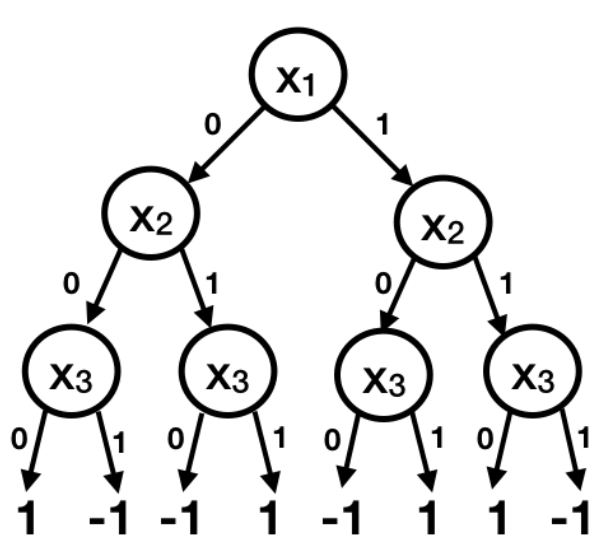
\includegraphics[width=0.25\textwidth]{report/figs/decision_tree.png}
        \label{fig:decision_tree}
    }
    \subfigure[]{
        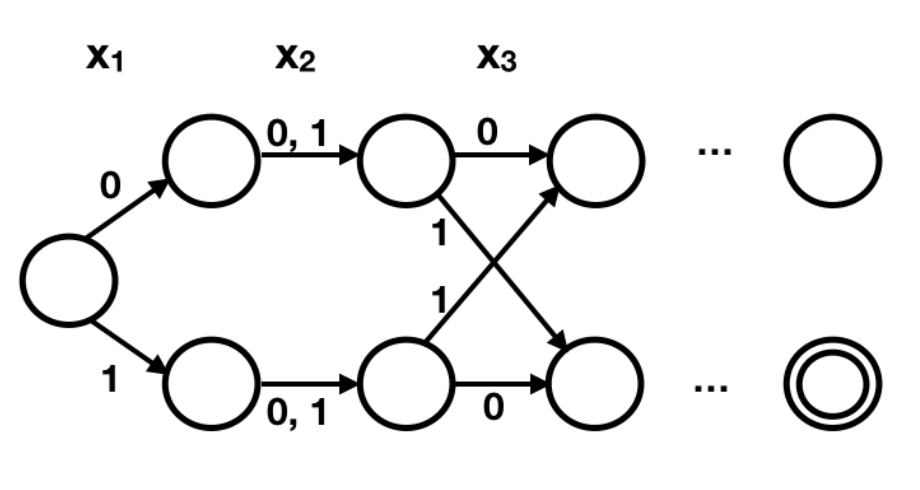
\includegraphics[width=0.4\textwidth]{report/figs/dfa.png}
        \label{fig:dfa}
    }
    \caption{(a) A decision tree with $7$ nodes encoding a parity function of size $3$ (b) A deterministic finite automata with $2n + 1$ nodes encoding a parity function of size $n$}
\end{figure*}
 
% \begin{figure}
%     \centering
%     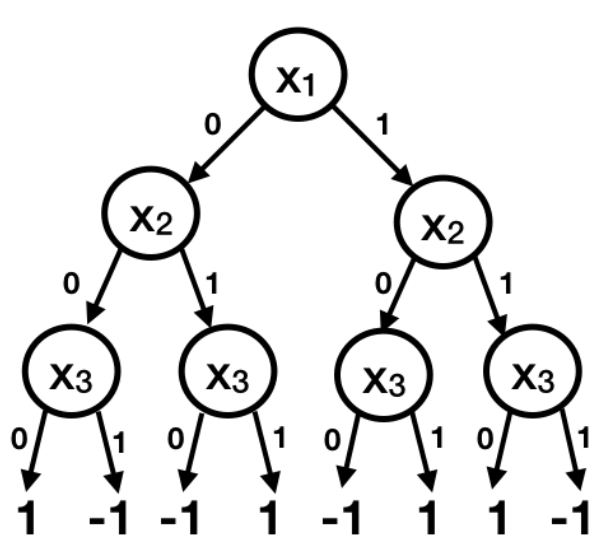
\includegraphics[width=0.4\textwidth]{report/figs/decision_tree.png}
%     \caption{A decision tree with $7$ nodes encoding a parity function of size $3$}
%     \label{fig:decision_tree}
% \end{figure}

\begin{proposition}
Disjunctive normal form (DNF) expressions of size $n$ have SQ-DIM $\geq n^{c.log(n)}$, and therefore, are not efficiently SQ learnable.
\end{proposition}

Like decision trees, DNF formulae can also be encoded by parity functions. The following is a $4$-term DNF encoded by a parity function of size $3$.
\begin{align*}
    (x_1 \wedge x_2 \wedge x_3) \vee (\overline{x_1} \wedge \overline{x_2} \wedge \overline{x_3}) \vee (\overline{x_1} \wedge x_2 \wedge \overline{x_3}) \vee (\overline{x_1} \wedge \overline{x_2} \wedge x_3)
\end{align*}

\begin{proposition}
Deterministic finite automata with $n$ nodes have SQ-DIM $\geq 2^{c.n}$, and therefore, are not efficiently SQ learnable.
\end{proposition}

As shown in Figure \ref{fig:dfa}, deterministic finite automata with $2n+1$ nodes can also encode a parity function of size $n$.

% \begin{figure}
%     \centering
%     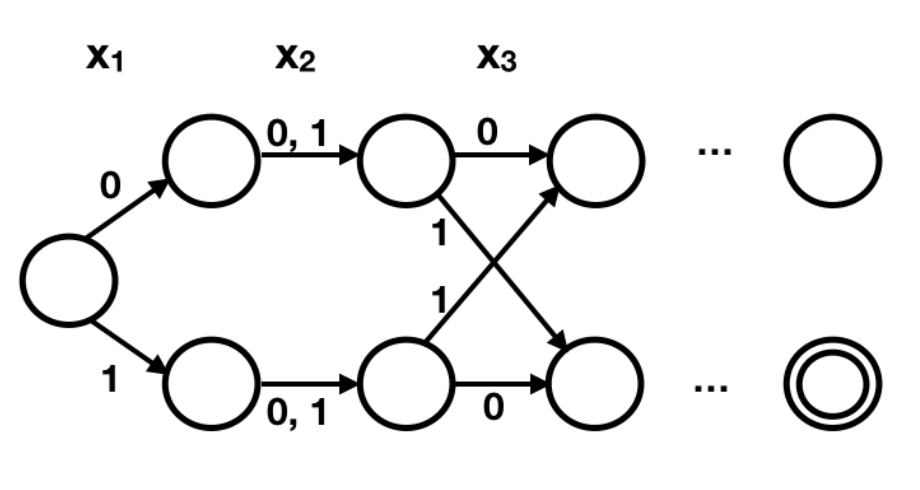
\includegraphics[width=0.4\textwidth]{report/figs/dfa.png}
%     \caption{A deterministic finite automata with $2n + 1$ nodes encoding a parity function of size $n$}
%     \label{fig:dfa}
% \end{figure}

\subsection{Complexity of learning}
Based on the above discussion, we can write the following hierarchy of models that contain the classes of functions that are learnable in those respective models:
\begin{align*}
    \text{efficient SQ} \subseteq \text{efficient PAC under classification noise} \subseteq \text{efficient PAC}
\end{align*}

\section{Learning Rectangle Problem using SQ}
\label{sec:implementation}

In this section, we implement an algorithm to learn the rectangle problem introduced in \cite{blumer_learnability_1989} using a statistical query oracle. The objective is to learn an unknown axis-aligned target rectangle $R$ which forms the boundary between a set of points in the Euclidean plane $\R^2$. The points inside the rectangle are positive examples and the ones outside are negative. Figure \ref{fig:rectangle_problem} shows the target rectangle $R$ along with a sample of positive and negative examples.

\begin{figure}
    \centering
    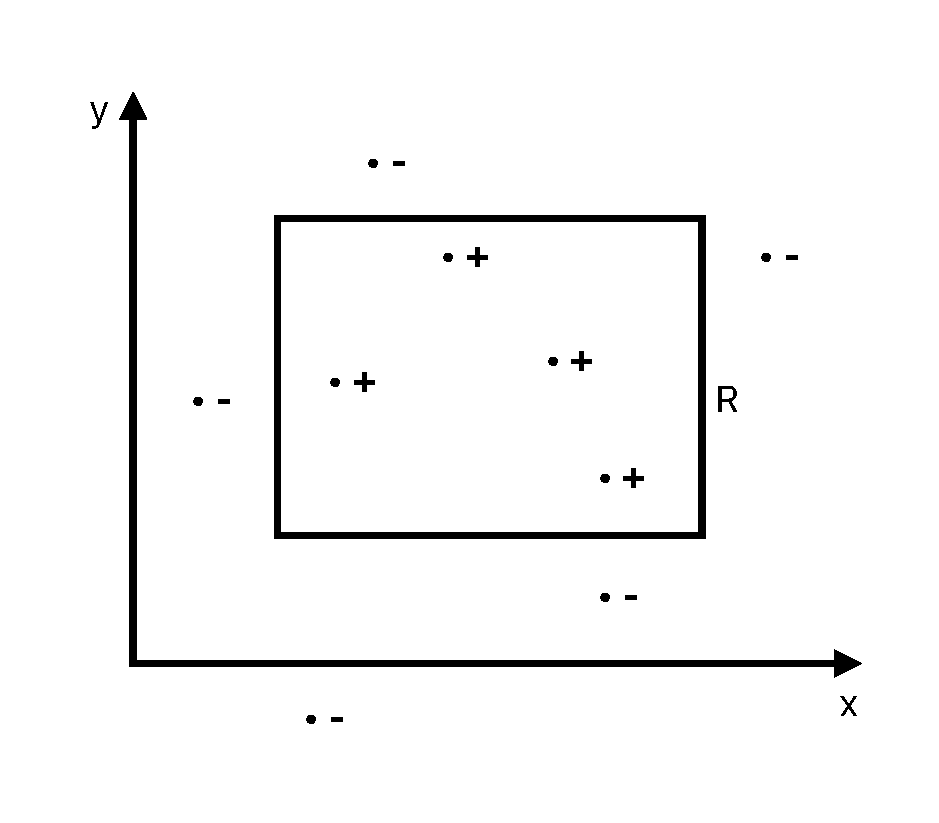
\includegraphics[width=0.36\textwidth]{report/figs/Rectangle.pdf}
    \caption{The target rectangle $R$ along with a sample of positive and negative examples \cite{kearns_introduction_1994}}
    \label{fig:rectangle_problem}
\end{figure}

To solve this problem using the statistical query learning framework, first, we define our concept class $C: \R^2 \xrightarrow{} \{-1, 1\}$, the statistical query $\chi: \R^2 \times \{-1, 1\} \xrightarrow{} \{-1, 1\}$ and the statistical query oracle $SQ(c, \cD)$. The statistical query oracle when given a function $c \in C$, will return an estimate of the expectation of whether the current hypothesis rectangle is correctly separating the positive and negative points $\nu: |\nu - \mathbb{E}_{\cD}[\chi(x, c(x))]| \leq \tau$. Now, we propose an algorithm to solve this problem using the defined statistical query oracle.

\begin{algorithm}[!h]
\caption{Rectangle Problem using SQ}
\label{rectangle_algo}
\begin{algorithmic}[1]
% \State $i \gets 10$
\State Input $SQ, \epsilon, min, max, \delta$
\State Initialize $c$ randomly to be a valid rectangle
\State Initialize $\nu \gets \infty, \Delta, c'$
\While{$|1 - \nu| > \epsilon$}
    \State $\Delta \gets Random(min, max, (max-min)*\delta)$
    \State $c' \gets c$
    \If{$Random(0, 1) < 0.5$}
        \State Change lower-left point by of $c'$ by $\Delta$
    \Else
        \State Change upper-right point of $c'$ by $\Delta$
    \EndIf
    \If{$c'$ is not valid}
        \State Skip to next iteration
    \EndIf
    % \If{$Random(0, 1) < 0.5$}
    %     \If{$Random(0, 1) < 0.5$}
    %         \State Increase $c'$ along x-axis by $w.\delta$
    %     \Else
    %         \State Decrease $c'$ along x-axis by $w.\delta$
    %     \EndIf
    % \Else
    %     \If{$Random(0, 1) < 0.5$}
    %         \State Increase $c'$ along y-axis by $w.\delta$
    %     \Else
    %         \State Decrease $c'$ along y-axis by $w.\delta$
    %     \EndIf
    % \EndIf
    \State $\nu' \gets SQ(c')$
    \If{$|1-\nu'| < |1-\nu|$}
        \State $\nu \gets \nu'$
        \State $c \gets c'$
    \EndIf
\EndWhile
\State Output $c$
\end{algorithmic}    
\end{algorithm}

\subsection{Algorithm}

Since each valid rectangle can be represented by two points, the lower-left point and the upper-right point, Algorithm \ref{rectangle_algo} changes either of these with equal probability. The change is based on some hyperparameters of the algorithm, $\epsilon, min, max \text{ and } \delta$. $\epsilon$ is the maximum error of the resultant hypothesis. $min \text{ and } max$ describe the minimum and maximum value we can take along the two axes. There is also another hyperparameter $\tau$ which is part of the statistical query oracle and it defines how close the estimate provided by the oracle is to the true value. The $Random$ function of Line 5 gives a random number in the range defined by $min \text{ and } max$ with the step size of $(max-min)*\delta$. To check whether a rectangle $c'$ is valid (Line 11), we check whether the points are in the range defined by $min \text{ and } max$, and if the values of the upper-right point along both the axes are greater than the lower-left point.

% Algorithm \ref{rectangle_algo} changes either of the two axes of the rectangle by a small value. It then checks with the statistical query oracle to see if the new rectangle estimate is better than the previous estimate. It loops through this process until the error of our rectangle estimate is better than $\epsilon$.

\subsection{Analysis}
\label{algo_analysis}
Algorithm \ref{rectangle_algo} does a random search over all the possible axis-aligned rectangles in the constraints defined by $min, max \text{ and } \delta$. In this section, we find an estimate of the number of these rectangles which is equal to the worst-case number of queries to the oracle. The region defined by these constraints will have roughly $\frac{1}{\delta^2}$ number of points from which we can choose the two points for a valid rectangle. The upper bound on the number of rectangles in this region can be given by $^{\frac{1}{\delta^2}}C_2 = \frac{1-\delta^2}{2.\delta^4} = O(\delta^{-4})$. Section \ref{app:algo_analysis} contains some results on the experiments conducted using the proposed algorithm.

\section{Conclusion}
\label{sec:conclusion}
In this report, we defined the statistical query oracle and how it can be used to develop noise-tolerant algorithms. We characterized how the statistical query framework relates to the PAC learning framework. Using the bounds of the statistical query algorithm we saw how some classes cannot be learned using statistical queries. In the end, we proposed an algorithm that uses the statistical query framework to solve the rectangle problem.


% \lipsum[75]

% \lipsum[5]

% \subsection{Motivation}
% \label{sec:motivation}
% \lipsum[66]

% \lipsum[5]

\bibliographystyle{plainnat} % We choose the "plain" reference style
\bibliography{refs} % Entries are in the refs.bib file
% \printbibliography

% \appendix

\appendix

\section{Additional Details}
\subsection{Correction Factor}
\label{correction_factor}
$\hat{P}_{noise}$ is the probability that a sample $x \in X$ can have noise in its label and $\eta$ is the noise or probability that a label is flipped. Also, let P be the true probability that a label is 1, then we can consider two scenarios
\begin{itemize}
    \item The true label is 1 and is not flipped $\left(P(1-\eta)\right)$
    \item The true label is 0 and is flipped $\left((1-P)\eta\right)$
\end{itemize}
\begin{align*}
    \hat{P}_{noise} &= P(1-\eta) + (1-P)\eta \\
    \hat{P}_{noise} &= P - P\eta + \eta - P\eta \\
    \hat{P}_{noise} - \eta &= P(1 - 2\eta) \\
    P &= \frac{\hat{P}_{noise} - \eta}{1 - 2\eta} \\
\end{align*}

This value is the correction factor and represents the proportion of labels that are not affected by the label noise.

\subsection{Algorithm Results}
\label{app:algo_analysis}
In this section, we give the results of the experiments conducted using the algorithm proposed in Section \ref{sec:implementation}. We conducted three types of experiments by varying $\epsilon, \tau \text{ and } \eta$. For each of the experiments, we fixed $min=-100 \text{ and } max=100$. We run each algorithm $150$ times to reduce the effect of stochasticity. Figure \ref{fig:results} shows the average number of statistical queries used by the algorithm for each of the different values of $\delta^{-1}$ along with $95\%$ confidence interval. For the first experiment, we varied the value of $\epsilon$, and kept $\tau$ and $\eta$ fixed at $0.1$ and $0.05$, respectively. Figure \ref{fig:epsilon} shows that for bigger values of $\epsilon$ it takes fewer queries to converge which was expected as convergence is faster for more error. For the second experiment, we varied $\tau$ and fixed $\epsilon=0.05$ and $\eta=0.05$. As shown in Figure \ref{fig:tau}, for $\tau=0$ it took comparatively too many queries for the algorithm to converge. This might be because for $\tau=0$ the algorithm became very prone to the noise in the data. For the last experiment, we varied $\eta$, and kept $\epsilon=0.05$ and $\tau=0.1$. In this case, as noise increased more queries were needed by the algorithm to find the hypothesis function. The algorithm also took very few queries in the noise-free situation (Figure \ref{fig:eta}). The analysis given in Section \ref{algo_analysis} gave the theoretical upper bound for the random search algorithm but it is worth noting that the experimental results show that the resultant algorithm is comparatively very optimal. This is because the proposed algorithm even though it initializes the initial hypothesis function randomly and searches through the concept class randomly but the search is guided by the output of the statistical query oracle ($\nu$). Based on $\nu$, the hypothesis function is only updated when the resultant change will make it closer to the resultant rectangle, in turn, making the algorithm efficient.

\begin{figure*}
    \centering
    \subfigure[]{
        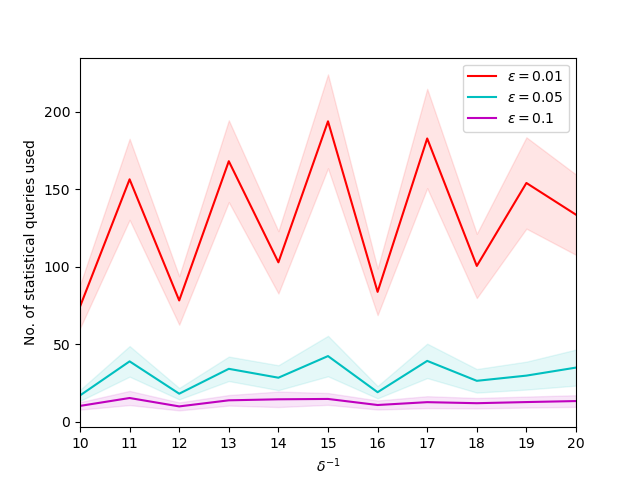
\includegraphics[width=0.48\textwidth]{report/figs/epsilon.png}
        \label{fig:epsilon}
    }
    \subfigure[]{
        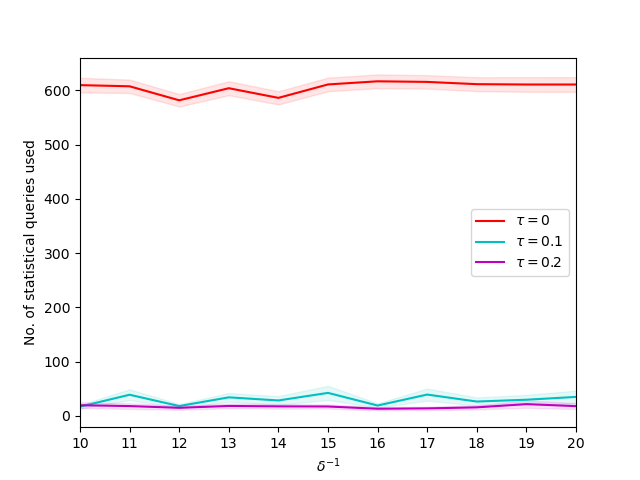
\includegraphics[width=0.48\textwidth]{report/figs/tau.png}
        \label{fig:tau}
    }
    \subfigure[]{
        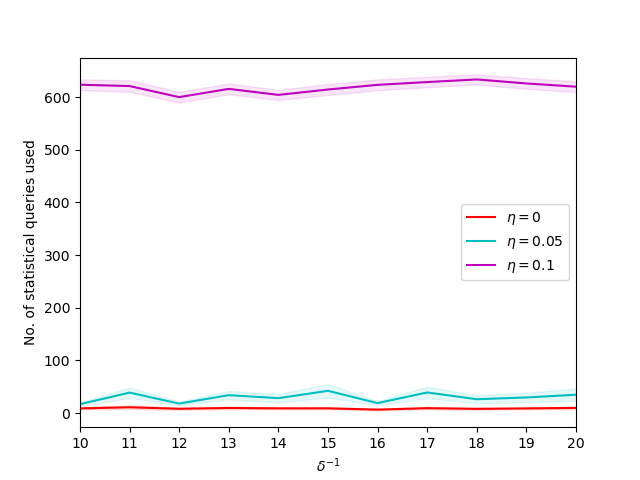
\includegraphics[width=0.48\textwidth]{report/figs/eta.png}
        \label{fig:eta}
    }
    \caption{Number of queries needed by the algorithm for (a) $\epsilon \in \{0.01, 0.05, 0.1\}, \tau=0.1, \eta=0.05$ (b) $\tau \in \{0, 0.1, 0.2\}, \epsilon=0.05, \eta=0.05$ (c) $\eta \in \{0, 0.05, 0.1\}, \epsilon=0.05, \tau=0.1$}
    \label{fig:results}
\end{figure*}

% \section{Additional Details}
% \label{backg}
% \subsection{Transformers}
% The architecture comprises stacked blocks that employ self-attention to process input sequences.

\end{document}
